\begin{frame}
\frametitle{Regularized potential}

Extracting an \emph{analytical} cusp from the wave function
\footcite{Seelig_1966}$^,$\footcite{Bischoff_2014a}
\begin{itemize}
    \item Nuclear correlation factor $R$
    \item Numerical exponential molecular orbital (NEMO) $F_i$
\end{itemize}

\vspace{5mm}

\centering
\textbf{Wave function ansatz}
\begin{equation}
    \nonumber
    \ket{\phi_i} = R\ket{F_i}
\end{equation}
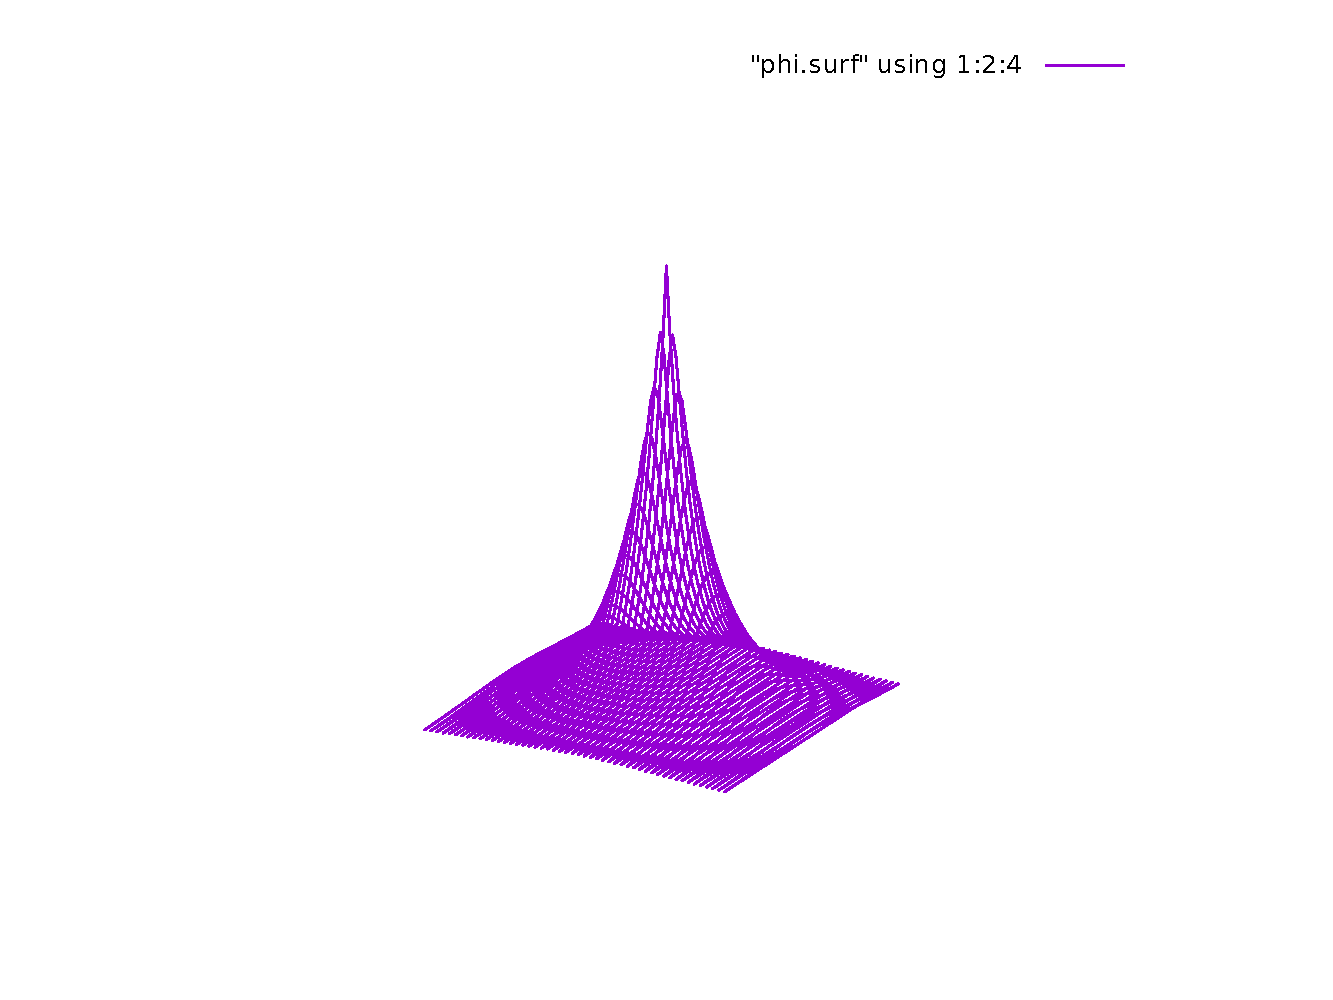
\includegraphics[scale=0.35, viewport = 175 90 430 400, clip]{figures/phi.pdf}
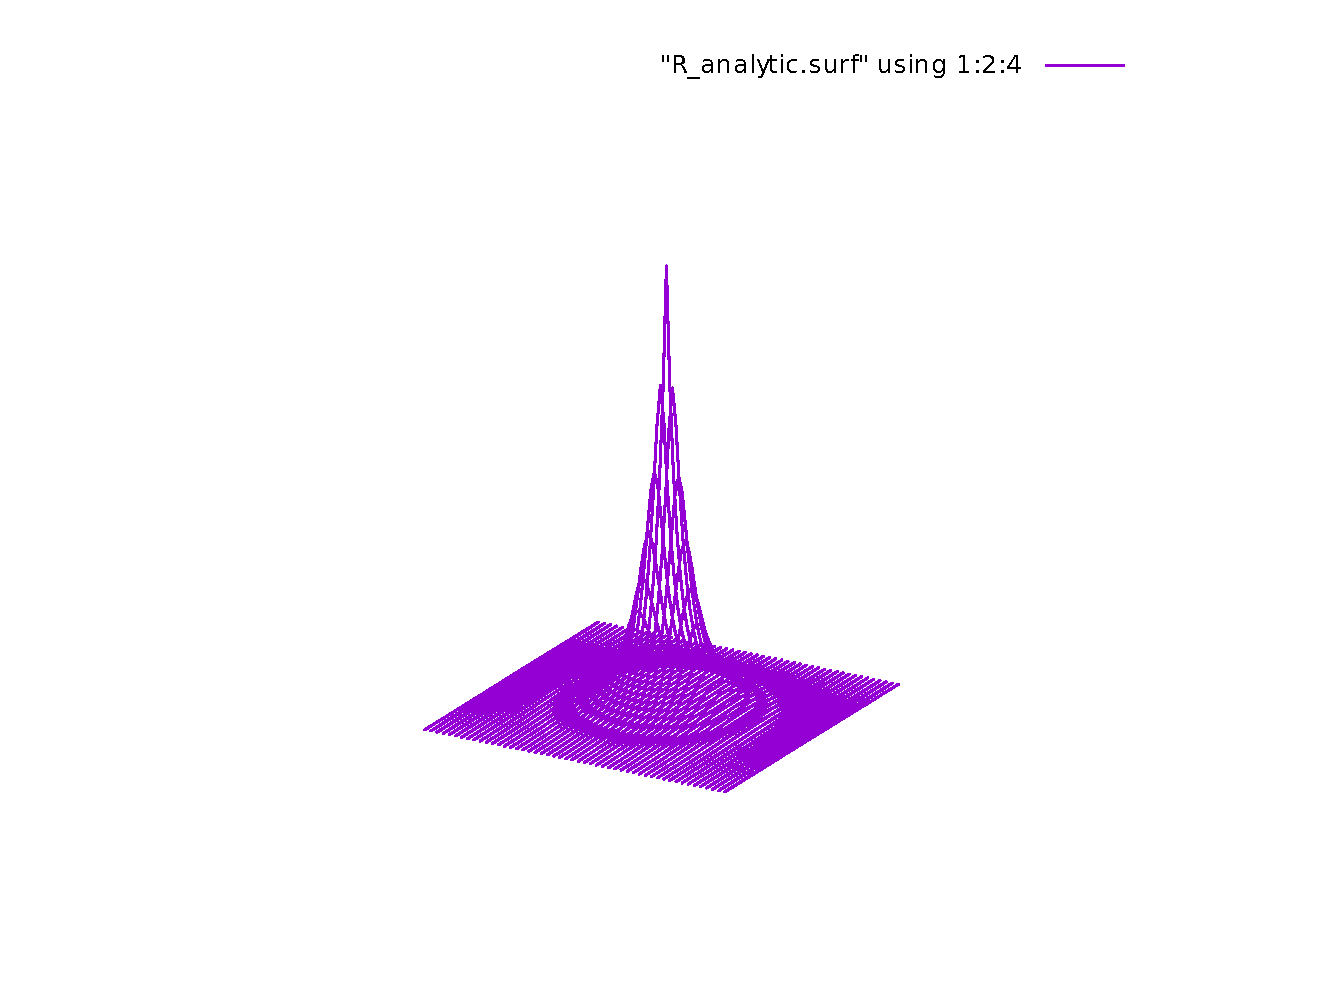
\includegraphics[scale=0.35, viewport = 175 90 430 400, clip]{figures/R.pdf}
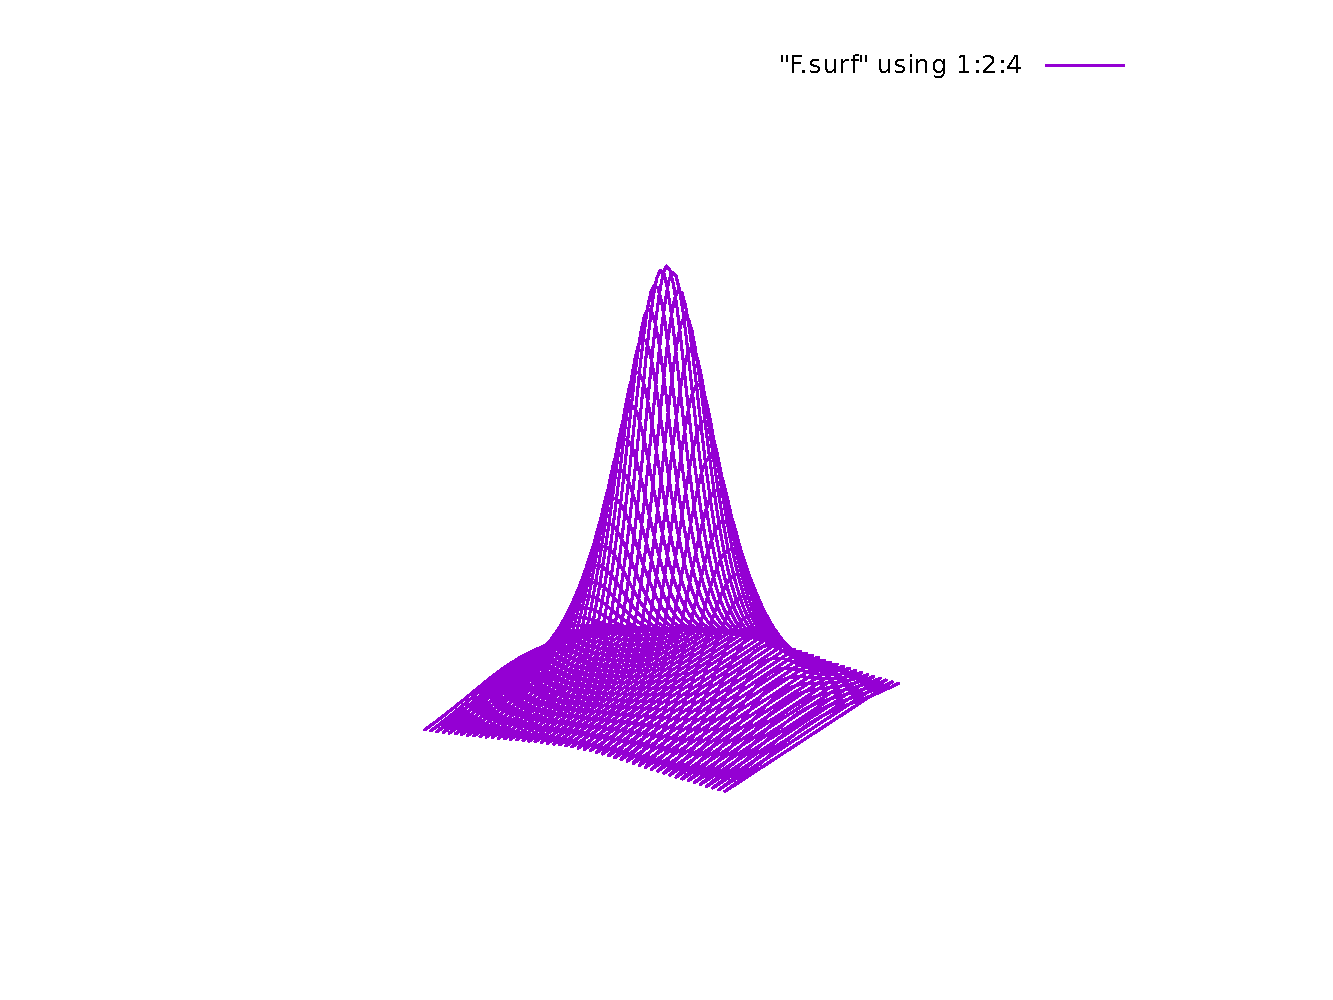
\includegraphics[scale=0.35, viewport = 175 90 430 400, clip]{figures/F.pdf}\\
\end{frame}

\begin{frame}
\frametitle{Regularized potential}
\centering

\textbf{Hartree-Fock equations}
\begin{equation}
    \nonumber
    \Big(T + V_{nuc} + J - K - \epsilon_i\Big)R\ket{F_i} = 0
\end{equation}

\vspace{5mm}

\pause
\textbf{Commuting the correlation factor to the left}
\begin{equation}
    \nonumber
    R\Big(T + R^{-1}[T,R] + V_{nuc} + J - R^{-1}KR - \epsilon_i\Big)\ket{F_i} = 0
\end{equation}

\vspace{5mm}

\pause
\textbf{Similarity transformed equations}
\begin{equation}
    \nonumber
    \Big(T + U_{nuc} + J - K_R - \epsilon_i\Big)\ket{F_i} = 0
\end{equation}
\begin{equation}
    \nonumber
    U_{nuc} = V_{nuc} + R^{-1}[T,R]
\end{equation}
\begin{equation}
    \nonumber
    K_R = R^{-1}KR
\end{equation}

\end{frame}

\usebackgroundtemplate{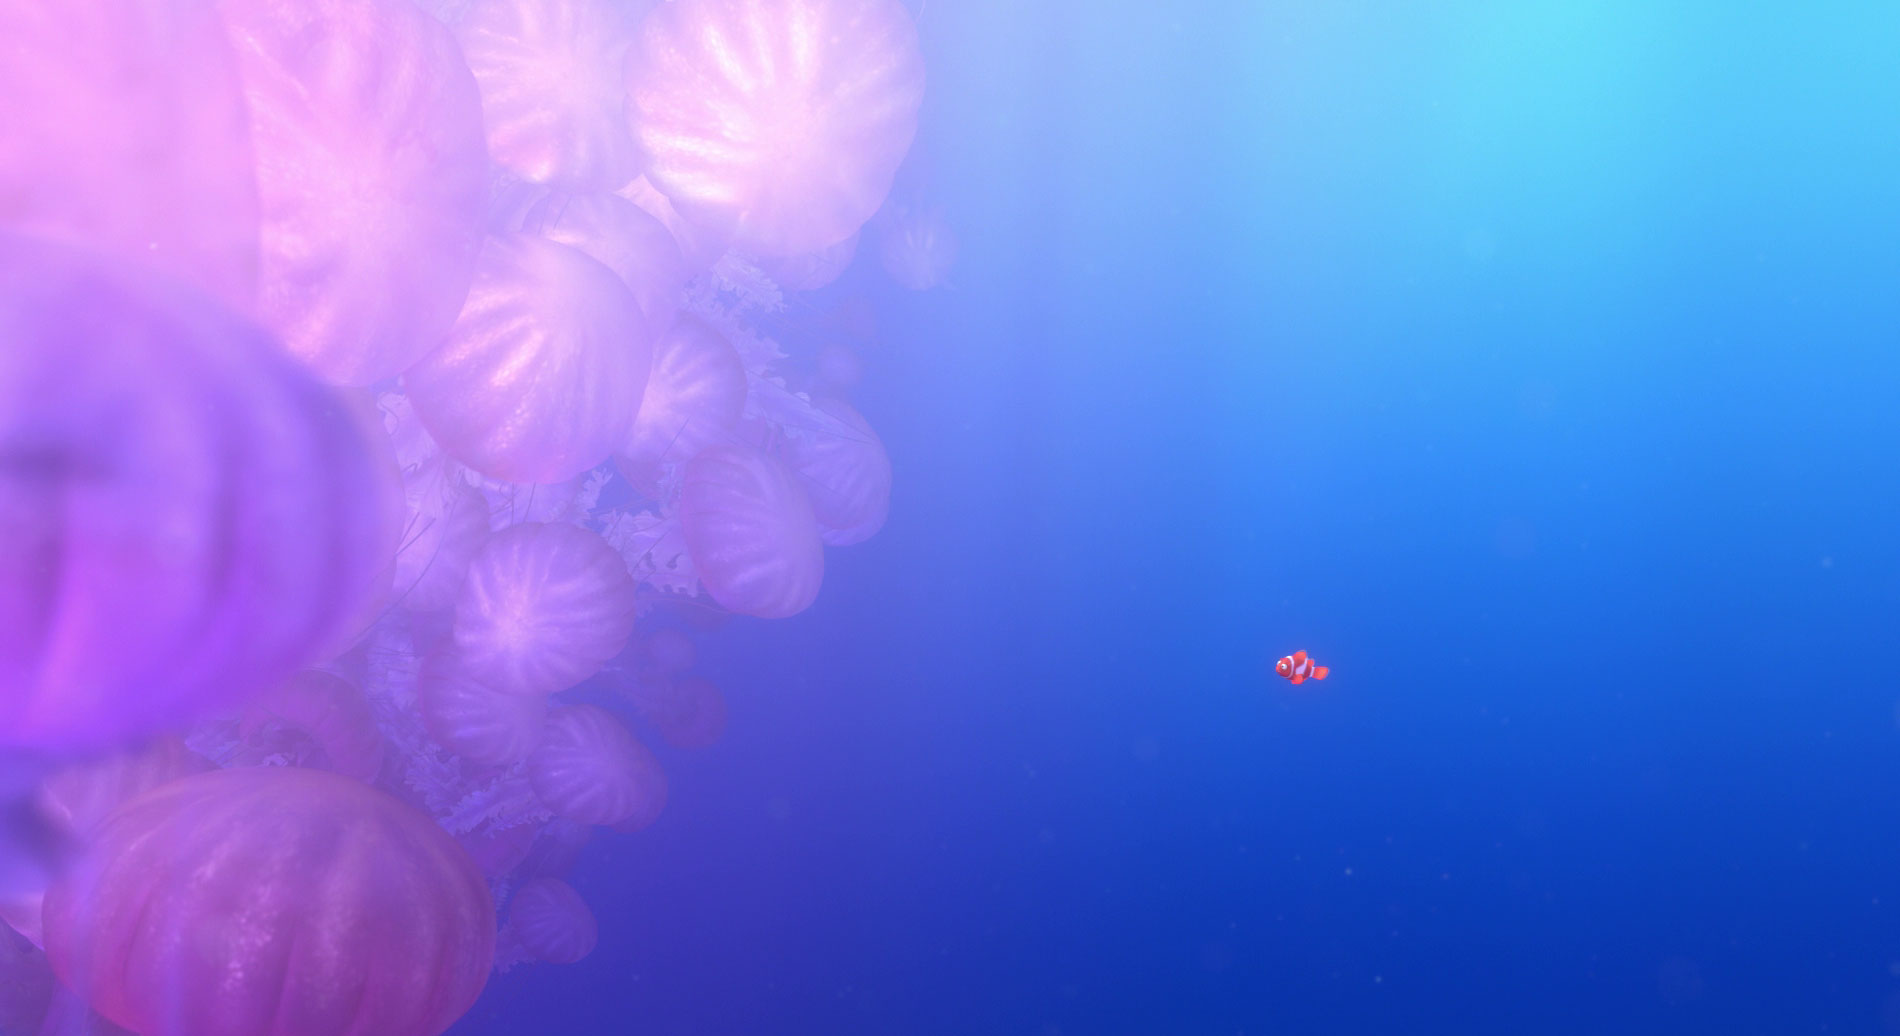
\includegraphics[scale=0.45, viewport=550 280 1400 900, clip]{figures/nemo_background.jpeg}}

\begin{frame}
\frametitle{Finding NEMO}
\scriptsize

\centering
\textbf{Transformed nuclear potential}
\centering
\begin{align}
    \nonumber
    U_{nuc} &=  V_{nuc} + R^{-1}[T,R]
             =  \Big(-\frac{Z}{r}\Big) + \Big(- \frac{\vec{R}^{'}}{R}\cdot\vec{\nabla}
                -\frac{1}{2}\frac{R^{''}}{R}\Big)
\end{align}

\vspace{5mm}

\begin{columns}
\begin{column}{.5\textwidth}

\pause
\centering
\only<1>{

\vspace{42.5mm}

}
\only<2,3,4>{
\textbf{Seelig's NEMO}
\begin{align}
    \nonumber
    R &= e^{-Zr}\\
    \nonumber
    -\frac{\vec{R}^{'}}{R} &= Z\vec{n}\\
    \nonumber
    -\frac{R^{''}}{R} -\frac{Z}{r} &= Z^2
\end{align}
}

\vspace{5mm}

\pause
\only<2>{

\vspace{12.5mm}

}
\only<3,4>{
\textbf{Regularized potential}
\begin{align}
    \nonumber
    U_{nuc} &=  Z\vec{n}\cdot\vec{\nabla} + \frac{Z^2}{2}
\end{align}
}
\end{column}

\begin{column}{.5\textwidth}
\centering
\only<4>{
\textbf{Slater NEMO}
\begin{equation}
    \nonumber
    R = 1 + \frac{e^{-aZr}}{a-1}
\end{equation}

\vspace{3mm}

\textbf{Gauss-Slater NEMO}
\begin{equation}
    \nonumber
    R = e^{-Zr} + \big(1 - e^{-Z^2r^2}\big)
\end{equation}

\vspace{3mm}

\textbf{Polynomial NEMO}
\begin{equation}
    \nonumber
    R = 1 + (-1)^na(-1+rZ/b)^n
\end{equation}
}

\end{column}
\end{columns}

\end{frame}

\usebackgroundtemplate{
\includegraphics[width=1.02\paperwidth]{figures/ctcc_general.jpg}}

\begin{frame}
\frametitle{One-electron system}
\centering

\textbf{Hydrogen atom}
\begin{equation}
    \nonumber
    \bigg(-\frac{\nabla^2}{2} - \frac{1}{r} \bigg)\phi(r) = \epsilon \phi(r)
\end{equation}

\pause
\vspace{10mm}

\textbf{Seelig's NEMO}
\begin{equation}
    \nonumber
    \phi(r) = R(r)F(r) = e^{-r}F(r)
\end{equation}

\pause
\vspace{10mm}

\textbf{Similarity transformed Schr\"{o}dinger equation}
\begin{equation}
    \nonumber
    \bigg(-\frac{\nabla^2}{2} + \vec{n}\cdot\vec{\nabla} + \frac{1}{2}\bigg)F(r) =
    \epsilon F(r)
\end{equation}

\end{frame}

\begin{frame}
\frametitle{One-electron system}
\centering
\scriptsize
\begin{table}
\textbf{Function value of Hydrogen 1s orbital}
\begin{tabular}{cclcl}
\hline
\hline
\multicolumn{1}{c}{\textbf{Precision}}&
\multicolumn{1}{c}{$\phi(r_0)$}&
\multicolumn{1}{l}{Error}&
\multicolumn{1}{c}{$\phi(r_1)$}&
\multicolumn{1}{l}{Error}\\
\hline
\hspace{10mm}\ &\hspace{20mm}\     &\hspace{15mm}\  &\hspace{20mm}\      &\hspace{10mm}\  \\
               &                   &                &                    &                \\
               &                   &                &                    &                \\
               &                   &                &                    &                \\
               &                   &                &                    &                \\
               &                   &                &                    &                \\
               &                   &                &                    &                \\
               &                   &                &                    &                \\
               &                   &                &                    &                \\
               &                   &                &                    &                \\
               &                   &                &                    &                \\
               &                   &                &                    &                \\
               &                   &                &                    &                \\
               &                   &                &                    &                \\
               &                   &                &                    &                \\
               &                   &                &                    &                \\
               &                   &                &                    &                \\
\hline
\hline
\end{tabular}
\end{table}
\tiny
$r_0$ at the nucleus, $r_1$ at a random point away from the nucleus
\end{frame}

\begin{frame}
\frametitle{One-electron system}
\centering
\scriptsize
\begin{table}
\textbf{Function value of Hydrogen 1s orbital}
\begin{tabular}{cclcl}
\hline
\hline
\multicolumn{1}{c}{\textbf{Precision}}&
\multicolumn{1}{c}{$\phi(r_0)$}&
\multicolumn{1}{l}{Error}&
\multicolumn{1}{c}{$\phi(r_1)$}&
\multicolumn{1}{l}{Error}\\
\hline
\hspace{10mm}\ &\hspace{20mm}\     &\hspace{15mm}\  &\hspace{20mm}\      &\hspace{10mm}\  \\
\multicolumn{5}{c}{R=Identity}\\
 MW4           &0.5\red{72 116 507}&   \red{7.9e-03}&0.474 3\red{87 750} & \green{7.6e-05}\\
 MW5           &0.56\red{6 687 228}&   \red{2.4e-03}&0.474 46\red{8 244} & \green{4.4e-06}\\
 MW6           &0.56\red{5 279 010}&   \red{1.0e-03}&0.474 464 \red{272} & \green{5.0e-07}\\
 MW7           &0.564 \red{553 287}&   \red{3.6e-04}&0.474 463 7\red{58} & \green{8.4e-09}\\
 MW8           &0.564 \red{252 177}&   \red{6.2e-05}&0.474 463 767       & \green{2.3e-10}\\
 Exact         &0.564 189 583      &-               &0.474 463 767       &-               \\
               &                   &                &                    &                \\
               &                   &                &                    &                \\
               &                   &                &                    &                \\
               &                   &                &                    &                \\
               &                   &                &                    &                \\
               &                   &                &                    &                \\
               &                   &                &                    &                \\
               &                   &                &                    &                \\
               &                   &                &                    &                \\
\hline
\hline
\end{tabular}
\end{table}
\tiny
$r_0$ at the nucleus, $r_1$ at a random point away from the nucleus
\end{frame}

\begin{frame}
\frametitle{One-electron system}
\centering
\scriptsize
\begin{table}
\textbf{Function value of Hydrogen 1s orbital}
\begin{tabular}{cclcl}
\hline
\hline
\multicolumn{1}{c}{\textbf{Precision}}&
\multicolumn{1}{c}{$\phi(r_0)$}&
\multicolumn{1}{l}{Error}&
\multicolumn{1}{c}{$\phi(r_1)$}&
\multicolumn{1}{l}{Error}\\
\hline
\hspace{10mm}\ &\hspace{20mm}\     &\hspace{15mm}\  &\hspace{20mm}\      &\hspace{10mm}\  \\
\multicolumn{5}{c}{R=Identity}\\
 MW4           &0.5\red{72 116 507}&   \red{7.9e-03}&0.474 3\red{87 750} & \green{7.6e-05}\\
 MW5           &0.56\red{6 687 228}&   \red{2.4e-03}&0.474 46\red{8 244} & \green{4.4e-06}\\
 MW6           &0.56\red{5 279 010}&   \red{1.0e-03}&0.474 464 \red{272} & \green{5.0e-07}\\
 MW7           &0.564 \red{553 287}&   \red{3.6e-04}&0.474 463 7\red{58} & \green{8.4e-09}\\
 MW8           &0.564 \red{252 177}&   \red{6.2e-05}&0.474 463 767       & \green{2.3e-10}\\
 Exact         &0.564 189 583      &-               &0.474 463 767       &-               \\
               &                   &                &                    &                \\
\multicolumn{5}{c}{R=Slater}\\
 MW4           &0.563 \red{832 013}&\yellow{3.5e-04}&0.474 \red{144 473} &\yellow{3.1e-04}\\
 MW5           &0.564 18\red{8 317}& \green{1.2e-06}&0.474 463 \red{210} & \green{5.5e-07}\\
 MW6           &0.564 18\red{8 486}&\yellow{1.0e-06}&0.474 462 \red{851} & \green{9.1e-07}\\
 MW7           &0.564 189 5\red{60}& \green{2.2e-08}&0.474 463 7\red{56} & \green{1.1e-08}\\
 MW8           &0.564 189 57\red{6}& \green{7.0e-09}&0.474 463 76\red{2} & \green{4.9e-09}\\
 Exact         &0.564 189 583      &-               &0.474 463 767       &-               \\
               &                   &                &                    &                \\
\hline
\hline
\end{tabular}
\end{table}
\tiny
$r_0$ at the nucleus, $r_1$ at a random point away from the nucleus
\end{frame}

\begin{frame}
\frametitle{Extension to more electrons}
\centering
\textbf{All orbitals share the same correlation factor}
\begin{equation}
    \nonumber
    \phi_i(r) = R(r) F_i(r)
\end{equation}

\end{frame}

%\begin{frame}
%\frametitle{Many-electron systems}
%\centering
%\begin{table}
%\textbf{Spin densities of the Fluorine atom (Unrestricted Hartree-Fock)}
%\begin{tabular}{crrr}
%\hline
%\hline
%\multicolumn{1}{c}{\textbf{Precision}}&
%\multicolumn{1}{c}{$\rho^\alpha(r_0)$}&
%\multicolumn{1}{c}{$\rho^\beta(r_0)$}&
%\multicolumn{1}{c}{$\rho^{\alpha-\beta}(r_0)$}\\
%\hline
%\hspace{10mm}\     & \hspace{20mm}\     & \hspace{20mm}\     & \hspace{15mm}\ \\
%                   &                    &                    &                \\
%                   &                    &                    &                \\
%                   &                    &                    &                \\
%                   &                    &                    &                \\
%                   &                    &                    &                \\
%                   &                    &                    &                \\
%                   &                    &                    &                \\
%                   &                    &                    &                \\
%                   &                    &                    &                \\
%                   &                    &                    &                \\
%                   &                    &                    &                \\
%                   &                    &                    &                \\
%                   &                    &                    &                \\
%                   &                    &                    &                \\
%\hline
%\hline
%\end{tabular}
%\end{table}
%\tiny
%$r_0$ at the nucleus
%\end{frame}
%
%\begin{frame}
%\frametitle{Many-electron systems}
%\centering
%\begin{table}
%\textbf{Spin densities of the Fluorine atom (Unrestricted Hartree-Fock)}
%\begin{tabular}{crrr}
%\hline
%\hline
%\multicolumn{1}{c}{\textbf{Precision}}&
%\multicolumn{1}{c}{$\rho^\alpha(r_0)$}&
%\multicolumn{1}{c}{$\rho^\beta(r_0)$}&
%\multicolumn{1}{c}{$\rho^{\alpha-\beta}(r_0)$}\\
%\hline
%\hspace{10mm}\     & \hspace{20mm}\     & \hspace{20mm}\     & \hspace{15mm}\ \\
%\multicolumn{4}{c}{R = Identity}\\
%               MW4 & 22\red{7.422 438}  & 22\red{7.286 520}  & 0.1\red{35 917}\\
%               MW5 & 22\red{5.108 976}  & 22\red{4.978 719}  & 0.13\red{0 256}\\
%               MW6 & 224.\red{595 243}  & 224.\red{464 582}  & 0.13\red{0 660}\\
%               MW7 & 224.\red{339 158}  & 224.\red{213 024}  & 0.12\red{6 134}\\
%               MW8 & 224.2\red{14 420}  & 224.0\red{89 374}  & 0.125 \red{046}\\
%                   &                    &                    &                \\
%                   &                    &                    &                \\
%                   &                    &                    &                \\
%                   &                    &                    &                \\
%                   &                    &                    &                \\
%                   &                    &                    &                \\
%                   &                    &                    &                \\
%                   &                    &                    &                \\
%\hline
%\hline
%\end{tabular}
%\end{table}
%\tiny
%$r_0$ at the nucleus
%\end{frame}

\begin{frame}
\frametitle{Extension to more electrons}
\centering
\begin{table}
\textbf{Spin densities of the Fluorine atom (Unrestricted Hartree-Fock)}
\begin{tabular}{crrr}
\hline
\hline
\multicolumn{1}{c}{\textbf{Precision}}&
\multicolumn{1}{c}{$\rho^\alpha(r_0)$}&
\multicolumn{1}{c}{$\rho^\beta(r_0)$}&
\multicolumn{1}{c}{$\rho^{\alpha-\beta}(r_0)$}\\
\hline
\hspace{10mm}\     & \hspace{20mm}\     & \hspace{20mm}\     & \hspace{15mm}\ \\
\multicolumn{4}{c}{R = Identity}\\
               MW4 & 22\red{7.422 438}  & 22\red{7.286 520}  & 0.1\red{35 917}\\
               MW5 & 22\red{5.108 976}  & 22\red{4.978 719}  & 0.13\red{0 256}\\
               MW6 & 224.\red{595 243}  & 224.\red{464 582}  & 0.13\red{0 660}\\
               MW7 & 224.\red{339 158}  & 224.\red{213 024}  & 0.12\red{6 134}\\
               MW8 & 224.2\red{14 420}  & 224.0\red{89 374}  & 0.125 \red{046}\\
                   &                    &                    &                \\
\multicolumn{4}{c}{R = Slater}\\
               MW4 & 223.\red{971 607}  & 223.\red{841 617}  & 0.12\red{9 990}\\
               MW5 & 224.1\red{91 162}  & 224.0\red{65 489}  & 0.125 \red{673}\\
               MW6 & 224.212 \red{732}  & 224.087 \red{100}  & 0.125 6\red{31}\\
               MW7 & 224.213 07\red{7}  & 224.087 44\red{0}  & 0.125 63\red{7}\\
               MW8 & 224.213 085        & 224.087 447        & 0.125 638      \\
                   &                    &                    &                \\
\hline
\hline
\end{tabular}
\end{table}
\tiny
$r_0$ at the nucleus
\end{frame}

\begin{frame}
\frametitle{Extension to more electrons}
\centering
\textbf{HFCC of the Fluorine atom (Unrestricted Hartree-Fock)}
\begin{table}
\begin{tabular}{rrrr}
\hline
\hline
\multicolumn{1}{r}{\textbf{GTO}}&
\multicolumn{1}{c}{A$_{FC}$ (MHz)}&
\multicolumn{1}{r}{\textbf{GTO}}&
\multicolumn{1}{c}{A$_{FC}$ (MHz)}\\
\hline
  cc-pVDZ      & \red{831.451}  &  cc-pCVDZ      & \red{ 53.566}  \\
  cc-pVTZ      & \red{  1.981}  &  cc-pCVTZ      & \red{429.481}  \\
  cc-pVQZ      & \red{144.487}  &  cc-pCVQZ      & 5\red{09.140}  \\
  cc-pV5Z      & \red{362.384}  &  cc-pCV5Z      & 51\red{5.986}  \\
\hline
\hline
\hspace{15mm}\ & \hspace{15mm}\ & \hspace{25mm}\ & \hspace{15mm}\ \\
\hspace{15mm}\ & \hspace{15mm}\ & \hspace{25mm}\ & \hspace{15mm}\ \\
\hline
\hline
\multicolumn{1}{r}{\textbf{GTO}}&
\multicolumn{1}{c}{A$_{FC}$ (MHz)}&
\multicolumn{1}{r}{\textbf{MRA}}&
\multicolumn{1}{c}{A$_{FC}$ (MHz)}\\
\hline
  pcJ-1         & 4\red{97.794}  &  MW5          & 5\red{47.641}  \\
  pcJ-2         & 5\red{13.137}  &  MW6          & 5\red{49.746}  \\
  pcJ-3         & 52\red{9.493}  &  MW7          & 53\red{0.701}  \\
  pcJ-4         & 528.\red{068}  &  MW8          & 52\red{5.862}  \\
\hline
\hline
\end{tabular}
\end{table}
\tiny
GTO calculations with ORCA\\
MWx: Multiwavelets with precision $\epsilon=10^{-x}$
\end{frame}


\begin{frame}
\frametitle{Extension to more electrons}
\centering
\textbf{HFCC of the Fluorine atom (Unrestricted Hartree-Fock)}
\begin{table}
\begin{tabular}{rrrr}
\hline
\hline
\multicolumn{1}{r}{\textbf{GTO}}&
\multicolumn{1}{c}{A$_{FC}$ (MHz)}&
\multicolumn{1}{r}{\textbf{GTO}}&
\multicolumn{1}{c}{A$_{FC}$ (MHz)}\\
\hline
  cc-pVDZ      & \red{831.451}  &  cc-pCVDZ      & \red{ 53.566}  \\
  cc-pVTZ      & \red{  1.981}  &  cc-pCVTZ      & \red{429.481}  \\
  cc-pVQZ      & \red{144.487}  &  cc-pCVQZ      & 5\red{09.140}  \\
  cc-pV5Z      & \red{362.384}  &  cc-pCV5Z      & 51\red{5.986}  \\
\hline
\hline
\hspace{15mm}\ & \hspace{15mm}\ & \hspace{25mm}\ & \hspace{15mm}\ \\
\hspace{15mm}\ & \hspace{15mm}\ & \hspace{25mm}\ & \hspace{15mm}\ \\
\hline
\hline
\multicolumn{1}{r}{\textbf{GTO}}&
\multicolumn{1}{c}{A$_{FC}$ (MHz)}&
\multicolumn{1}{r}{\textbf{MRA}}&
\multicolumn{1}{c}{A$_{FC}$ (MHz)}\\
\hline
  pcJ-1         & 4\red{97.794}  &  MW5           &52\red{6.972}  \\
  pcJ-2         & 5\red{13.137}  &  MW6           &528.\red{482}  \\
  pcJ-3         & 52\red{9.493}  &  MW7           &528.61\red{3}  \\
  pcJ-4         & 528.\red{068}  &  MW8           &528.619        \\
\hline
\hline
\end{tabular}
\end{table}
\tiny
GTO calculations with ORCA\\
MWx: Multiwavelets with precision $\epsilon=10^{-x}$
\end{frame}

\begin{frame}
\frametitle{Extension to more nuclei}
\centering
\textbf{All orbitals share the same correlation factor}
\begin{equation}
    \nonumber
    \phi_i(r) = R(r) F_i(r)
\end{equation}

\vspace{10mm}

\textbf{All nuclei are combined into one correlation factor}
\begin{equation}
    \nonumber
    R(r) = \prod_I R_I(r - r_I)
\end{equation}

\end{frame}

\begin{frame}
\frametitle{Extension to more nuclei}
\centering
\textbf{Isotropic (Fermi-Contact) contribution to HFCC}
\begin{equation}
    \nonumber
    A_{FC} = \Big(\frac{4\pi}{3}\langle S_z \rangle^{-1}\Big)
    g_eg_N\beta_e\beta_N\rho^{\alpha-\beta}(r_N)
\end{equation}

\begin{table}
\textbf{HFCC of O$_2$ molecule (PBE)}\\
\begin{tabular}{crrrr}
\hline
\hline
\multicolumn{1}{c}{\textbf{Precision}}&
\multicolumn{1}{c}{$A_{FC}(O1)$}&
\multicolumn{1}{c}{$A_{FC}(O2)$}&
\multicolumn{1}{c}{\textbf{GTO}}&
\multicolumn{1}{c}{$A_{FC}(O)$}\\
\hline
\hspace{10mm}\     & \hspace{18mm}\ & \hspace{18mm}\  &         & \hspace{18mm}\ \\
                   &\multicolumn{2}{c}{R = Identity}  &      pcJ-1 & -17.2393 \\
               MW4 & -\red{27.9573} &  -\red{9.6738}  &      pcJ-2 & -20.5463 \\
               MW5 & -\red{11.4636} & -20.\red{9434}  &      pcJ-3 & -21.1093 \\
               MW6 & -21.\red{3382} & -21.\red{0007}  &      pcJ-4 & -21.2139 \\
               MW7 & -21.\red{0051} & -21.\red{3342}  &     upcJ-4 & -21.2083 \\
               MW8 & -21.\red{1106} & -21.\red{2558}  &  aug-pcJ-4 & -21.2371 \\
                   &                &                 &                       \\
\hline
\hline
\end{tabular}
\end{table}
\tiny
O$_1$ at the origin, O$_2$ distance $|r|=1.2075$\AA\ from the origin\\
\ \\
GTO calculations with ORCA\\
MWx: Multiwavelets with precision $\epsilon=10^{-x}$\\
pcJ-x: Jensen's polarization-consistent (optimized for spin-spin coupling)
\end{frame}

\begin{frame}
\frametitle{Extension to more nuclei}
\centering
\textbf{Isotropic (Fermi-Contact) contribution to HFCC}
\begin{equation}
    \nonumber
    A_{FC} = \Big(\frac{4\pi}{3}\langle S_z \rangle^{-1}\Big)
    g_eg_N\beta_e\beta_N\rho^{\alpha-\beta}(r_N)
\end{equation}

\begin{table}
\textbf{HFCC of O$_2$ molecule (PBE)}\\
\begin{tabular}{crrrr}
\hline
\hline
\multicolumn{1}{c}{\textbf{Precision}}&
\multicolumn{1}{c}{$A_{FC}(O1)$}&
\multicolumn{1}{c}{$A_{FC}(O2)$}&
\multicolumn{1}{c}{\textbf{GTO}}&
\multicolumn{1}{c}{$A_{FC}(O)$}\\
\hline
\hspace{10mm}\     & \hspace{18mm}\ & \hspace{18mm}\  &            & \hspace{18mm}\ \\
                   &\multicolumn{2}{c}{R = Slater}    &      pcJ-1 & -1\red{7.2393} \\
               MW4 & -21.\red{8971} & -21.\red{9006}  &      pcJ-2 & -20.\red{5463} \\
               MW5 & -20.\red{9662} & -20.\red{9805}  &      pcJ-3 & -21.1\red{093} \\
               MW6 & -21.0\red{824} & -21.0\red{687}  &      pcJ-4 & -21.\red{2139} \\
               MW7 & -21.07\red{32} & -21.07\red{21}  &     upcJ-4 & -21.\red{2083} \\
               MW8 & -21.071\red{3} & -21.071\red{7}  &  aug-pcJ-4 & -21.\red{2371} \\
                   &                &                 &                             \\
\hline
\hline
\end{tabular}
\end{table}
\tiny
O$_1$ at the origin, O$_2$ distance $|r|=1.2075$\AA\ from the origin\\
\ \\
GTO calculations with ORCA\\
MWx: Multiwavelets with precision $\epsilon=10^{-x}$\\
pcJ-x: Jensen's polarization-consistent (optimized for spin-spin coupling)
\end{frame}

